\documentclass[%
reprint,
%superscriptaddress,
%groupedaddress,
%unsortedaddress,
%runinaddress,
%frontmatterverbose, 
%preprint,
%preprintnumbers,
nofootinbib,
%nobibnotes,
%bibnotes,
 amsmath,amssymb,
aps,
%pra,
%prb,
%rmp,
%prstab,
%prstper,
%floatfix,
superscriptaddress,
showkeys,
%endfloats,
%onecolumn,
longbibliography
]{revtex4-1}

%TESTE
\usepackage{enumitem}

\usepackage{xr}
\usepackage{tabularx}
\usepackage{booktabs}
\usepackage{graphicx}% Include figure files
\usepackage{dcolumn}% Align table columns on decimal point
\usepackage{bm}% bold math
\usepackage{microtype}
\usepackage{gensymb}
\usepackage{url}
% Permitir inclusão de PDFs com versão mais alta no output (não resolve a inclusão em si)
\pdfminorversion=7
\pdfobjcompresslevel=0
% add hypertext capabilities e evitar duplicação de anchors
\usepackage[breaklinks, hidelinks, colorlinks=true,linkcolor=blue,citecolor=black,hypertexnames=false]{hyperref}
\usepackage{color, colortbl}
\usepackage[table,xcdraw]{xcolor}
%\usepackage[mathlines]{lineno}% Enable numbering of text and display math
%\linenumbers\relax % Commence numbering lines

%\usepackage[showframe,%Uncomment any one of the following lines to test 
%%scale=0.7, marginratio={1:1, 2:3}, ignoreall,% default settings
%%text={7in,10in},centering,
%%margin=1.5in,
%%total={6.5in,8.75in}, top=1.2in, left=0.9in, includefoot,
%%height=10in,a5paper,hmargin={3cm,0.8in},
%]{geometry}

%VER
% (Removido xcolor duplicado)

\makeatletter
\renewcommand\frontmatter@abstractwidth{\dimexpr0.9\textwidth\relax}
\makeatother


% \bibliographystyle{apsrev4-1}
\usepackage{algorithm}
\usepackage{algpseudocode}
\usepackage{multirow}

\makeatletter
\newcommand*{\addFileDependency}[1]{% argument=file name and extension
  \typeout{(#1)}
  \@addtofilelist{#1}
  \IfFileExists{#1}{}{\typeout{No file #1.}}
}
\makeatother

\newcommand*{\myexternaldocument}[1]{%
    \externaldocument{#1}%
    \addFileDependency{#1.tex}%
    \addFileDependency{#1.aux}%
}

\newcommand{\sm}{\scalebox{0.5}[1.0]{\( - \)}}


%VER
\makeatletter
\renewcommand\subparagraph{\@startsection{subparagraph}{5}{\parindent}%
    {3.25ex \@plus1ex \@minus .2ex}%
    {-1em}%
    {\normalfont\normalsize\bfseries}}
\makeatother

\begin{document}

\preprint{1}



\title{VessShape: Few-shot 2D blood vessel segmentation by leveraging shape priors from synthetic images}
%VessShape: Few-shot blood vessel segmentation using shape priors from synthetic data
%VessShape: Adding shape priors to neural networks for few-shot blood vessel segmentation

\author{Wesley Nogueira Galvão}
\affiliation{Department of Computer Science, Federal University of S\~ao Carlos, S\~ao Carlos, SP, Brazil}


\author{Cesar H. Comin}
\email[Corresponding author: ]{comin@ufscar.br}
\affiliation{Department of Computer Science, Federal University of S\~ao Carlos, S\~ao Carlos, SP, Brazil}

\date{\today}% It is always \today, today,
             %  but any date may be explicitly specified

\begin{abstract}

??

\end{abstract}

\keywords{Blood vessel segmentation, Connectivity, post-processing}

\maketitle
\thispagestyle{plain}
%\ohead*{\pagemark}
\section{Metodologia}
\label{s:methodology}

\subsection{O conjunto de dados VessShape}

A geometria das imagens sintéticas é baseada em curvas de Bézier, que permitem uma representação flexível e controlada de formas tubulares. Cada segmento vascular é descrito por uma curva de Bézier de ordem $n$ com pontos de controle $\{\mathbf{p}_i\}_{i=0}^n$. A tortuosidade dos segmentos é ajustada por pequenas perturbações nos pontos de controle, garantindo que a geometria seja realista e diversificada. A curva de Bézier $\mathbf{c}(t)$ de um segmento é dada por

\begin{equation}
\mathbf{c}(t) \,=\, \sum_{i=0}^{n} \binom{n}{i} (1-t)^{n-i} t^{i} \, \mathbf{p}_i,
\label{eq:bezier}
\end{equation}
onde $t \in [0,1]$.

Para gerar uma curva, o primeiro ($\mathbf{p}_0$) e o último ($\mathbf{p}_n$) pontos de controle são sorteados com distribuição uniforme. Os demais $n-2$ pontos são inicialmente colocados de forma equiespaçada no segmento que liga $\mathbf{p}_0$ a $\mathbf{p}_n$ e depois deslocados por uma quantidade aleatória ao longo de um vetor normal unitário. O deslocamento é amostrado de $[-\delta,\delta]$. Valores menores de $\delta$ produzem segmentos mais retilíneos.

Para formar a máscara binária $M$, cada curva é amostrada em resolução suficiente e os pontos sucessivos são conectados formando uma polilinha de 1 pixel. Em seguida aplica-se dilatação morfológica com elemento estruturante disco de raio $r_0$, conferindo espessura tubular constante inicial antes de eventuais variações suaves.

Os parâmetros (número de segmentos $K$, ordem $n$, escala de deslocamento $\delta$ e raio $r_0$) são sorteados de intervalos predefinidos para maximizar a variabilidade geométrica. A Tabela~\ref{tab:vessshape_params} resume esses parâmetros.

\begin{table*}[t]
\caption{Principais parâmetros usados na geração do VessShape.}
\label{tab:vessshape_params}
\centering
\begin{tabularx}{\textwidth}{l c X}
\hline
    	extbf{Parâmetro} & \textbf{Intervalo} & \textbf{Descrição} \\
\hline
Número de curvas $K$ & $[1,20]$ & Quantidade de ramos/vasos por amostra. \\
Pontos de controle $n{+}1$ & $[2,20]$ & Complexidade (ordem $n$) da curva de Bézier. \\
Escala de deslocamento $\delta$ (px) & $[50.0,150.0]$ & Amplitude típica do deslocamento dos pontos de controle (tortuosidade). \\
Raio inicial $r_{0}$ (px) & $[1,5]$ & Espessura basal; aplica-se afilamento suave ao longo do ramo. \\
Desfoque de matting $\sigma$ & $[1,2]$ & Desvio padrão da Gaussiana para $A = G_{\sigma} * M$. \\
\hline
\end{tabularx}
\end{table*}

Para compor a imagem final $I$ a partir da máscara $M$, escolhem-se aleatoriamente duas texturas de classes distintas do ImageNet~\cite{JiaDeng2009}: uma de primeiro plano $F$ e uma de fundo $B$. Ambas são recortadas e redimensionadas para $H \times W$. Gera-se um matte $A$ aplicando filtro Gaussiano de desvio $\sigma$ sobre $M$ e normalizando para $[0,1]$. A composição é

\begin{equation}
I \,=\, A F + (1-A) B,
\label{eq:compose}
\end{equation}
de modo que regiões de vaso ($A \approx 1$) preservam $F$, enquanto o restante ($A \approx 0$) preserva $B$. O parâmetro $\sigma$ controla a suavidade das bordas. Após a composição, aplica-se normalização canal a canal usando estatísticas do ImageNet. Exemplos aparecem na Figura~\ref{f:vessshape_sample}.

\begin{figure}[tbp]
    \centering
    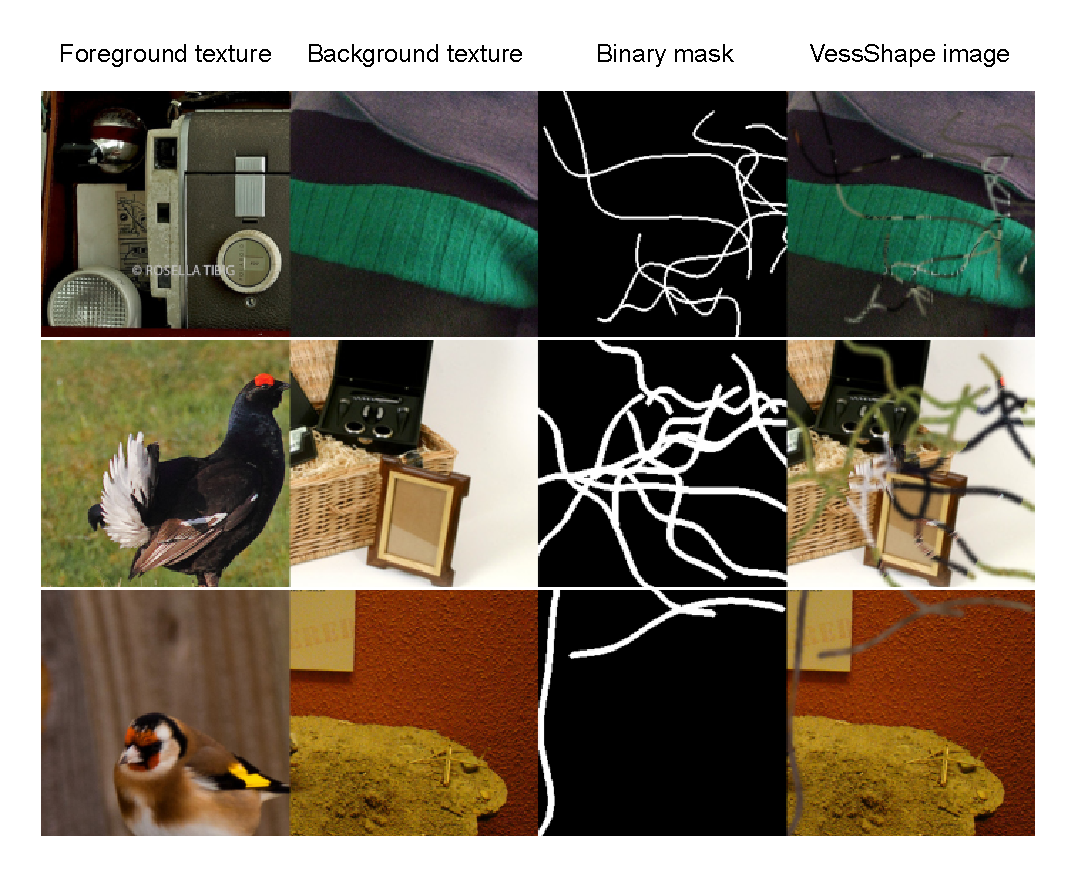
\includegraphics[width=\columnwidth]{figures/results/vessshape_sample.pdf}
    \caption{Exemplos de texturas do ImageNet, máscaras geométricas sintéticas e imagens resultantes VessShape.}
    \label{f:vessshape_sample}
\end{figure}

\subsection{Dados reais para validação}

Utilizamos os conjuntos DRIVE e VessMAP para avaliar a utilidade dos vieses de forma. DRIVE (40 imagens 584\,$\times$\,565, 20 treino / 20 teste) é referência para vasos de retina. VessMAP (100 imagens 256\,$\times$\,256 de microscopia de fluorescência cortical) apresenta ruído e contraste heterogêneos, múltiplos calibres e artefatos. As modalidades diferem: em VessMAP vasos brilhantes em fundo escuro; em DRIVE vasos escuros sobre fundo claro. Exemplos na Figura~\ref{f:drive_vessmap_samples}.

\begin{figure}[tbp]
    \centering
    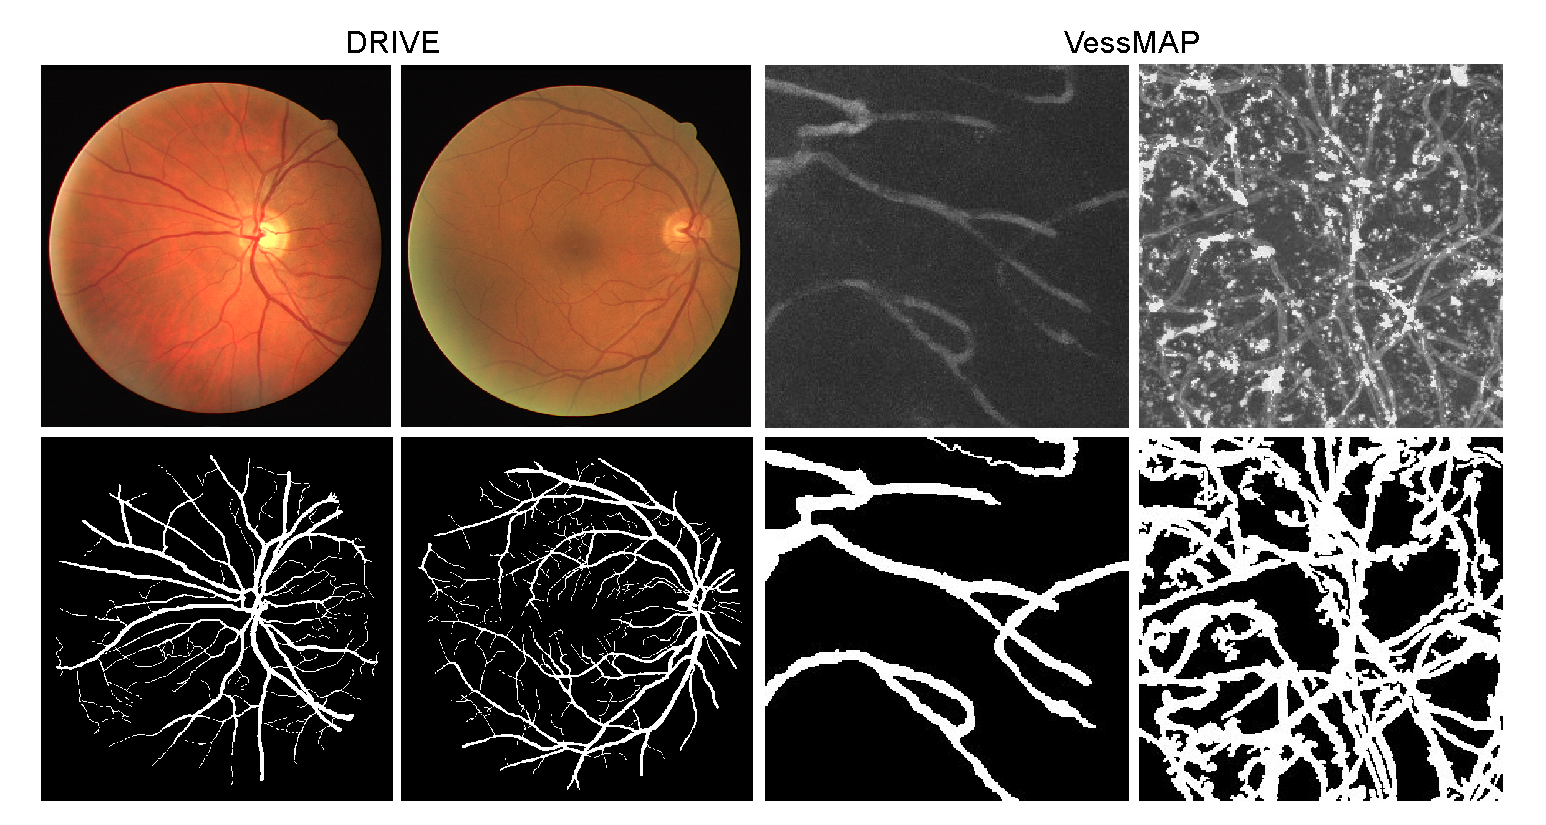
\includegraphics[width=\columnwidth]{figures/results/drive_vessmap_samples.pdf}
    \caption{Exemplos das bases DRIVE e VessMAP e respectivas máscaras anotadas.}
    \label{f:drive_vessmap_samples}
\end{figure}

\subsection{Arquitetura e estratégias de treinamento}

Adotamos arquitetura U-Net encoder–decoder com conexões de atalho. Comparamos variantes com encoders ResNet18 e ResNet50~\cite{he2016deep}, instanciadas via \textit{Segmentation Models Pytorch}\footnote{\url{https://github.com/qubvel/segmentation_models.pytorch}}.

Dois cenários: (i) treinamento do zero em DRIVE e VessMAP; (ii) pré-treinamento em VessShape seguido de fine-tuning. Assim, distinguimos três procedimentos: (a) training from scratch; (b) pre-training em VessShape; (c) fine-tuning nos dados reais.

\subsection{Pré-treinamento em VessShape}

O pré-treinamento busca expor o modelo a vasta diversidade geométrica com texturas variáveis como pista secundária, favorecendo recuperação de estruturas finas. Treinamos dois modelos (VSUNet18 e VSUNet50). A Tabela~\ref{tab:vs_hparams} resume hiperparâmetros.

\begin{table}[t]
    \caption{Hiperparâmetros de pré-treinamento no VessShape.}
    \label{tab:vs_hparams}
    \centering
    \begingroup
    \small
    \setlength{\tabcolsep}{6pt}
    \renewcommand{\arraystretch}{1.15}
    \begin{tabular}{l r r}
        \hline
        	extbf{Hiperparâmetro} & \textbf{VSUNet50} & \textbf{VSUNet18} \\
        \hline
        Batch size & 96 & 192 \\
        Learning rate & 1.0e-3 & 1.0e-2 \\
        LR decay & 0.0 & 0.0 \\
        Weight decay & 1.0e-4 & 0.0 \\
        Imgs/epoch & 50{,}000 & 50{,}000 \\
        Max epochs & 3000 & 1000 \\
        \hline
    \end{tabular}
    \endgroup
\end{table}

\subsection{Fine-tuning}

Após o pré-treinamento, os pesos são ajustados em subsets de DRIVE e VessMAP (cenários few-shot e full) para avaliar ganho de amostragem e transferência de forma.

\begin{table}[t]
    \caption{Desempenho das variantes VSUNet após pré-treinamento no VessShape.}
    \label{tab:vessshape_results}
    \centering
    \begingroup
    \small
    \setlength{\tabcolsep}{6pt}
    \renewcommand{\arraystretch}{1.15}
    \begin{tabular}{l r r}
        \hline
        	extbf{Métrica} & \textbf{VSUNet50} & \textbf{VSUNet18} \\
        \hline
        Dice & $0.861 \,\pm\, 0.022$ & $0.859 \,\pm\, 0.077$ \\
        Acc & $0.960 \,\pm\, 0.008$ & $0.956 \,\pm\, 0.037$ \\
        IoU & $0.758 \,\pm\, 0.032$ & $0.761 \,\pm\, 0.096$ \\
        Prec & $0.780 \,\pm\, 0.037$ & $0.774 \,\pm\, 0.096$ \\
        Rec & $0.964 \,\pm\, 0.012$ & $0.974 \,\pm\, 0.018$ \\
        \hline
    \end{tabular}
    \endgroup
\end{table}
Para gerar cada máscara binária, o número de segmentos $K$, a ordem $n$ das curvas de Bézier, a escala de deslocamento $\\delta$ e o raio $r_0$ são todos amostrados aleatoriamente de um intervalo para garantir uma ampla variedade de formas. A Tabela 
ef{tab:vessshape_params} resume os parâmetros usados na geração do conjunto de dados VessShape, juntamente com suas faixas de amostragem e descrições.

\begin{table*}[t]
\caption{Principais parâmetros usados para gerar o conjunto de dados VessShape.}
\label{tab:vessshape_params}
\centering
\begin{tabularx}{\textwidth}{l c X}
\hline
    \textbf{Parâmetro} & \textbf{Intervalo} & \textbf{Descrição} \\
\hline
Número de curvas $K$ & $[1,20]$ & Número de ramos/vasos gerados por amostra. \ 
Pontos de controle $n{+}1$ & $[2,20]$ & Complexidade da curva de Bézier (ordem $n$). \ 
Escala de deslocamento $\\delta$ (px) & $[50.0,150.0]$ & Controla a curvatura/tortuosidade através da amplitude típica do deslocamento do ponto de controle. \ 
Raio inicial $r_{0}$ (px) & $[1,5]$ & Espessura basal do vaso; um afilamento suave é aplicado ao longo do ramo. \ 
Borrão de matting $\\sigma$ & $[1,2]$ & Desvio padrão da Gaussiana usada para $A = G_{\\sigma} * M$. \ 

\hline
\end{tabularx}
\end{table*}

Para compor a imagem final $I$ a partir de uma máscara binária $M$, uma textura de primeiro plano $F$ e uma textura de fundo $B$ são inseridas, respectivamente, nos segmentos de vasos gerados e no fundo da imagem. As texturas são selecionadas aleatoriamente do ImageNet 
cite{JiaDeng2009}. Especificamente, para cada máscara $M$, duas imagens são sorteadas aleatoriamente de duas classes distintas do conjunto de dados ImageNet. As imagens são então cortadas e redimensionadas aleatoriamente para as dimensões alvo ($H \times W$). Uma máscara alfa $A$ é então gerada suavizando $M$ com um filtro Gaussiano de desvio padrão $\\sigma$ e normalizando seus valores para o intervalo $[0, 1]$. As texturas são subsequentemente misturadas usando esta máscara de acordo com

\begin{equation}
I \,=\, A\,F + (1-A)\,B,
\label{eq:compose}
\end{equation}
o que garante que as regiões dos vasos ($A \approx 1$) preservem o primeiro plano, enquanto as regiões não vasculares ($A \approx 0$) retenham o fundo.

O parâmetro $\\sigma$ controla a suavidade das bordas do vaso. Após a composição, a imagem $I$ passa por uma normalização por canal usando as estatísticas do ImageNet para compatibilidade com modelos pré-treinados. Exemplos de máscaras e imagens geradas são mostrados na Figura~
ef{f:vessshape_sample}.


\begin{figure}[tbp]
    \centering
    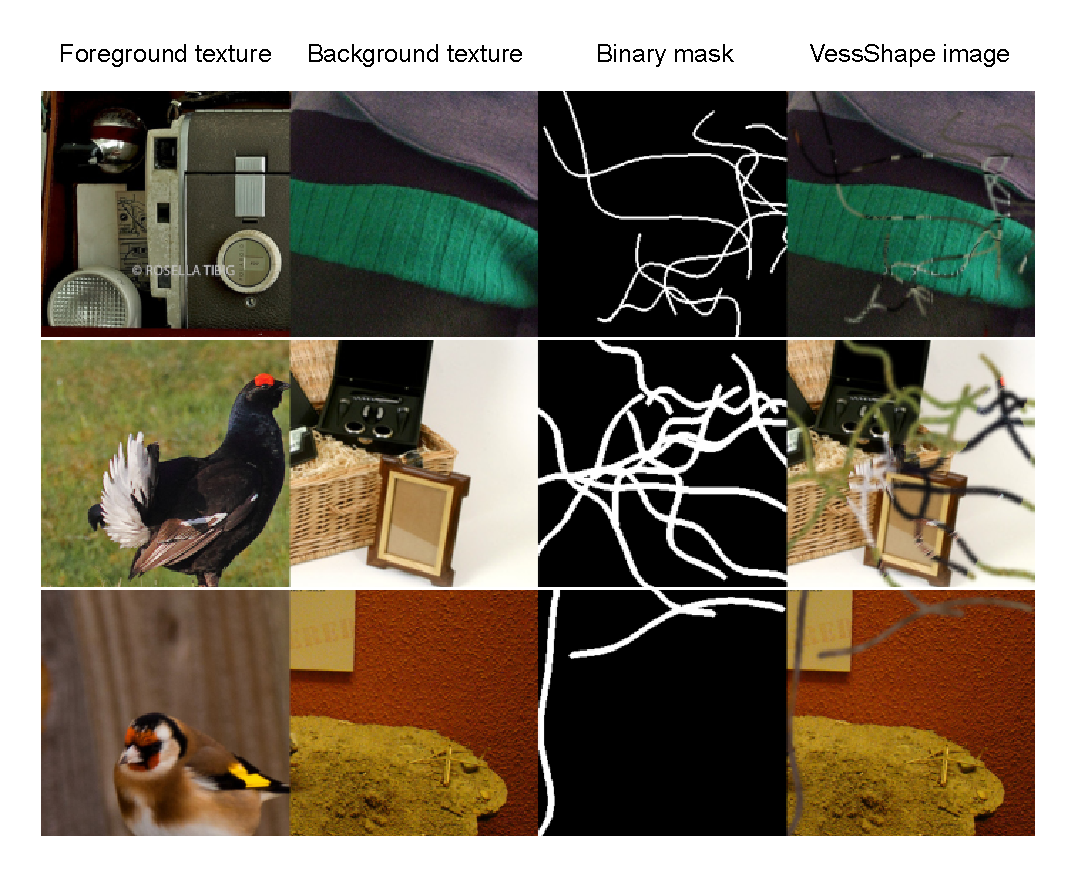
\includegraphics[width=\columnwidth]{figures/results/vessshape_sample.pdf}
    \caption{Exemplos de amostras do ImageNet, geometria sintética e respectivas imagens VessShape. As amostras do ImageNet são usadas como texturas para as máscaras binárias sintéticas, definindo a respectiva imagem VessShape.}
    \label{f:vessshape_sample}
\end{figure}

\subsection{Dados do mundo real para validação}

Para quantificar a utilidade do viés de forma introduzido pelo conjunto de dados VessShape, consideramos dois conjuntos de dados de vasos sanguíneos: DRIVE e VessMAP. O conjunto de dados DRIVE~
cite{} serve como um padrão popular para benchmarking de algoritmos de segmentação de vasos da retina e é composto por 40 fotografias de fundo de olho divididas em 20 para treinamento e 20 para teste, cada uma medindo 584×565 pixels. O conjunto de dados VessMAP consiste em 100 imagens, de 256×256 pixels cada, adquiridas por microscopia de fluorescência do córtex do camundongo. Ele foi curado para incluir uma variedade de características vasculares desafiadoras, como ruído e níveis de contraste inconsistentes, diferentes tamanhos de vasos, artefatos de imagem proeminentes e flutuações de intensidade dentro das estruturas vasculares.

Os dois conjuntos de dados originam-se de modalidades de imagem fundamentalmente diferentes, resultando em características distintas. As imagens de fundo de olho no DRIVE, que capturam toda a retina, possuem uma estrutura global clara que inclui marcos como o disco óptico. As amostras também contêm muitos vasos muito finos que são difíceis de segmentar. Em contraste, as imagens do VessMAP são visualizações altamente ampliadas de pequenas áreas corticais e não possuem organização global discernível. As bordas dos vasos são geralmente menos definidas do que os vasos do DRIVE. Outra diferença fundamental é que, sem qualquer processamento, os vasos no VessMAP são brilhantes com fundos escuros, enquanto os vasos no DRIVE são escuros com fundos brilhantes. A Figura 
ef{f:drive_vessmap_samples} mostra uma amostra de cada conjunto de dados.

\begin{figure}[tbp]
    \centering
    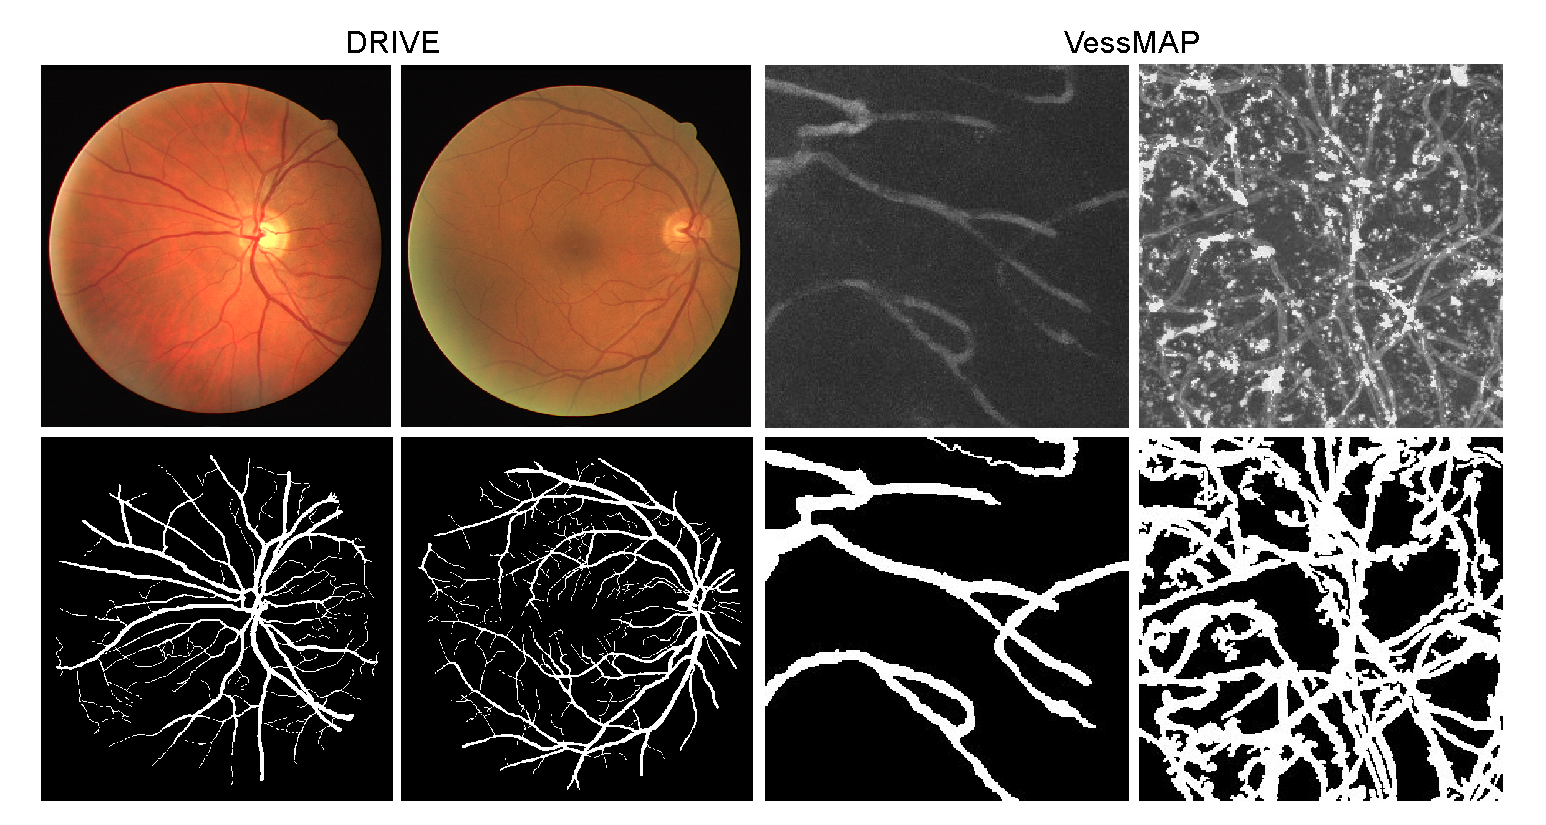
\includegraphics[width=\columnwidth]{figures/results/drive_vessmap_samples.pdf}
    \caption{Amostras dos conjuntos de dados DRIVE e VessMAP e suas respectivas máscaras de verdade do terreno.}
    \label{f:drive_vessmap_samples}
\end{figure}

\subsection{Arquiteturas de modelo e estratégias de treinamento}

Adotamos um design U-Net codificador-decodificador, ou seja, o decodificador é simétrico ao codificador e o modelo contém conexões de atalho entre diferentes estágios codificador-decodificador. Dois modelos são comparados, um com um codificador ResNet18 e outro com um codificador ResNet50 
cite{he2016deep}. Os modelos foram instanciados a partir do pacote Python 	extit{Segmentation Models Pytorch}\ootnote{\url{https://github.com/qubvel/segmentation_models.pytorch}}.

Dois cenários de treinamento são considerados. No primeiro, o treinamento é feito do zero separadamente nos conjuntos de dados DRIVE e VessMAP para estabelecer uma linha de base. O segundo cenário consiste em pré-treinar no conjunto de dados VessShape e ajustar fino no DRIVE e VessMAP para medir a transferibilidade e a eficiência da amostra das representações aprendidas. Esses dois cenários envolvem três procedimentos de treinamento distintos: i) treinamento do zero em conjuntos de dados naturais; ii) pré-treinamento no VessShape e iii) ajuste fino em dados do mundo real. Esses procedimentos são descritos a seguir.

\subsection{Treinamento do zero em conjuntos de dados naturais}

\subsection{Pré-treinamento no VessShape}

O pré-treinamento no VessShape visa expor o modelo a uma ampla variedade de geometrias tubulares, mantendo a textura como uma pista secundária, o que tende a beneficiar a segmentação de estruturas finas. O modelo é treinado para minimizar a perda média sobre um grande número de amostras extraídas do conjunto de dados sintético

Concretamente, pré-treinamos dois modelos U-Net, um com um codificador ResNet18 e outro com um codificador ResNet50. Nós nos referimos a eles como VSUNet18 e VSUNet50, respectivamente. O fluxo de treinamento expõe intencionalmente o modelo a geometrias do tipo vaso, enquanto as texturas continuam mudando no fundo. Essa narrativa de formas abundantes e aparências mutáveis ​​leva a rede a confiar menos em pistas de textura superficiais e mais em regularidades geométricas que importam para a conectividade e a recuperação de estruturas finas. Abaixo, detalhamos a configuração do VSUNet50 e resumimos seu desempenho no VessShape.

\begin{table}[t]
    \caption{Hiperparâmetros de pré-treinamento no VessShape.}
    \label{tab:vs_hparams}
    \centering
    \begingroup
    \small
    \setlength{\tabcolsep}{6pt}
    \renewcommand{\arraystretch}{1.15}
    \begin{tabular}{l r r}
        \hline
        \t\textbf{Hiperparâmetro} & \textbf{VSUNet50} & \textbf{VSUNet18} \\
        \hline
        Tamanho do lote & 96 & 192 \\
        Taxa de aprendizado & 1.0e-3 & 1.0e-2 \\
        Decaimento da taxa de aprendizado & 0.0 & 0.0 \\
        Decaimento de peso & 1.0e-4 & 0.0 \\
        Imgs/época & 50{,}\\!000 & 50{,}\\!000 \\
        Épocas máximas & 3000 & 1000 \\
        \hline
    \end{tabular}
    \endgroup
\end{table*}


\subsection{Ajuste fino em conjuntos de dados naturais}

- Conjuntos de dados (VessMAP e DRIVE)

- Procedimento

\begin{table}[t]
    \caption{Desempenho das variantes VSUNet após pré-treinamento no VessShape.}
    \label{tab:vessshape_results}
    \centering
    \begingroup
    \small
    \setlength{\tabcolsep}{6pt}
    \renewcommand{\arraystretch}{1.15}
    \begin{tabular}{l r r}
        \hline
        \t\textbf{Métrica} & \textbf{VSUNet50} & \textbf{VSUNet18} \\
        \hline
        Dice & $0.861 \,\pm\, 0.022$ & $0.859 \,\pm\, 0.077$ \\
        Acc & $0.960 \,\pm\, 0.008$ & $0.956 \,\pm\, 0.037$ \\
        IoU & $0.758 \,\pm\, 0.032$ & $0.761 \,\pm\, 0.096$ \\
        Prec & $0.780 \,\pm\, 0.037$ & $0.774 \,\pm\, 0.096$ \\
        Rec & $0.964 \,\pm\, 0.012$ & $0.974 \,\pm\, 0.018$ \\
        \hline
    \end{tabular}
    \endgroup
\end{table*}

\section{Resultados}
\label{s:results}

\begin{figure*}[tbp]
    \centering
    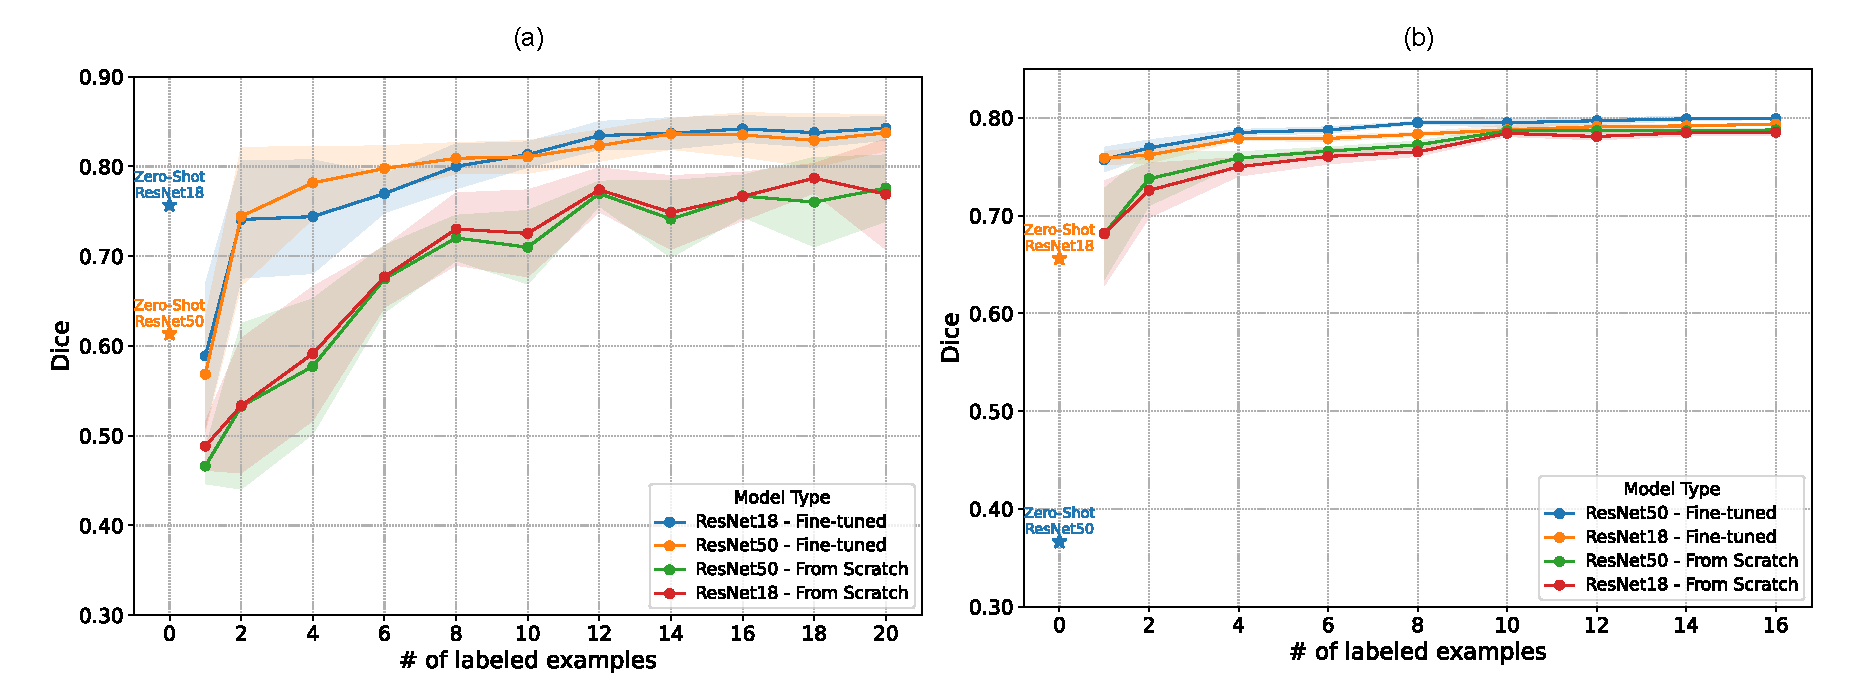
\includegraphics[width=\textwidth]{figures/results/results_charts.pdf}
    \caption{??.}
    \label{f:results_charts}
\end{figure*}


\begin{figure*}[tbp]
    \centering
    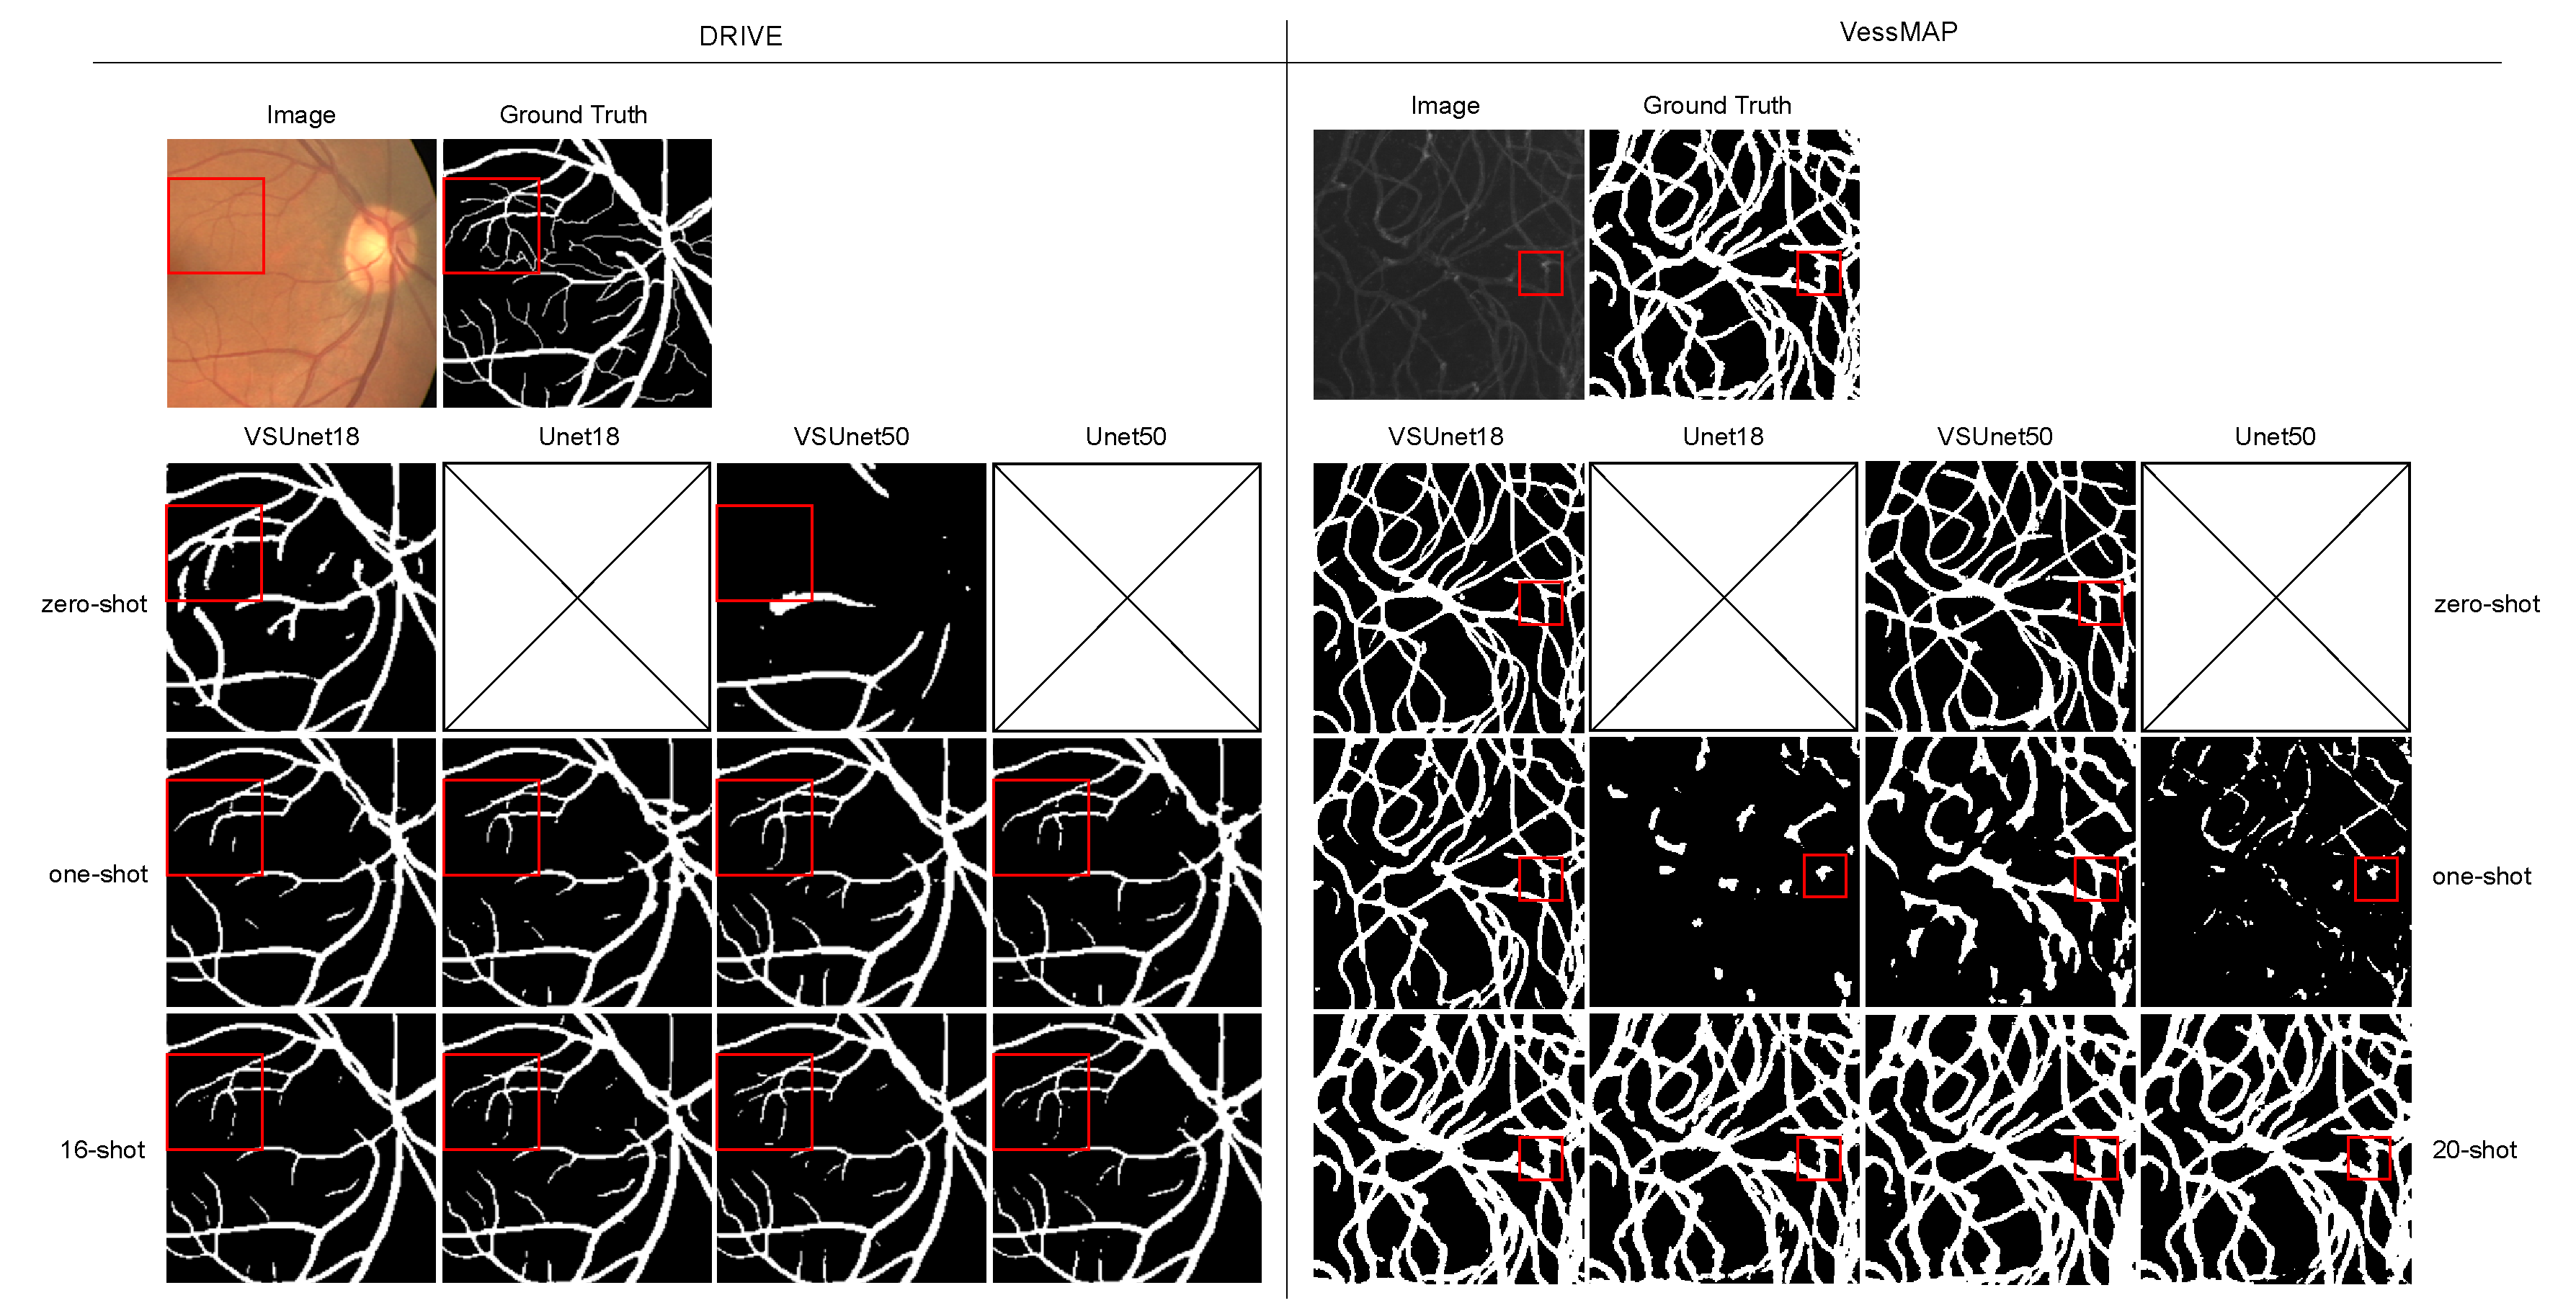
\includegraphics[width=\textwidth]{figures/results/results_fewshots.pdf}
    \caption{??.}
    \label{f:results_fewshots_drive}
\end{figure*}



% TODO:
% Argumentar que o nosso modelo é capaz de segmentar em zero-shot a forma do vaso, mesmo para VessMap que tem vasos com intensidade mais alta (branco), e DRIVE, com vasos com intensidade mais baixa(preto). 

% Tabela combinada de few-shot para VessMAP + DRIVE
\begin{table*}[t]
    \caption{Segmentação few-shot e zero-shot em VessMAP e DRIVE. Os valores são média $\pm$ desvio padrão sobre execuções repetidas (ajuste fino para modelos VSUNet e treinamento do zero para baselines U-Net) avaliados em cada conjunto de teste do conjunto de dados. As linhas de zero-shot vêm de uma única inferência pré-treinada (sem desvio disponível).}
    \label{tab:combined_fewshot}
    \centering
    \begingroup
    \small
    \setlength{\tabcolsep}{4pt}
    \renewcommand{\arraystretch}{1.15}
    % Coluna AUC removida; células de Dataset mescladas com multirow
    \begin{tabular}{l r l r r r r r}
        \hline
        \textbf{Conjunto de dados} & \textbf{\#Exemplos} & \textbf{Modelo} & \textbf{Dice} & \textbf{Acc} & \textbf{IoU} & \textbf{Prec} & \textbf{Rec} \\
        \hline
        \multirow{10}{*}{DRIVE} & \multirow{2}{*}{0} & VSUNet18 & $0.656 \,\pm\, 0.000$ & $0.907 \,\pm\, 0.000$ & $0.490 \,\pm\, 0.000$ & $0.629 \,\pm\, 0.000$ & $0.699 \,\pm\, 0.000$ \\
         &  & VSUNet50 & $0.367 \,\pm\, 0.000$ & $0.888 \,\pm\, 0.000$ & $0.230 \,\pm\, 0.000$ & $0.728 \,\pm\, 0.000$ & $0.275 \,\pm\, 0.000$ \\
         \cline{2-8}
         & \multirow{4}{*}{1} & VSUNet18 & $0.759 \,\pm\, 0.007$ & $0.941 \,\pm\, 0.002$ & $0.612 \,\pm\, 0.009$ & $0.787 \,\pm\, 0.021$ & $0.741 \,\pm\, 0.019$ \\
         &  & VSUNet50 & $0.757 \,\pm\, 0.013$ & $0.939 \,\pm\, 0.006$ & $0.611 \,\pm\, 0.016$ & $0.773 \,\pm\, 0.046$ & $0.754 \,\pm\, 0.039$ \\
         &  & UNet18 & $0.682 \,\pm\, 0.054$ & $0.919 \,\pm\, 0.016$ & $0.523 \,\pm\, 0.058$ & $0.717 \,\pm\, 0.079$ & $0.690 \,\pm\, 0.118$ \\
         &  & UNet50 & $0.681 \,\pm\, 0.046$ & $0.916 \,\pm\, 0.031$ & $0.523 \,\pm\, 0.050$ & $0.722 \,\pm\, 0.099$ & $0.690 \,\pm\, 0.110$ \\
         \cline{2-8}
         & \multirow{4}{*}{16} & VSUNet18 & $0.794 \,\pm\, 0.000$ & $0.950 \,\pm\, 0.000$ & $0.658 \,\pm\, 0.000$ & $0.833 \,\pm\, 0.004$ & $0.762 \,\pm\, 0.003$ \\
         &  & VSUNet50 & $0.799 \,\pm\, 0.001$ & $0.952 \,\pm\, 0.000$ & $0.666 \,\pm\, 0.001$ & $0.846 \,\pm\, 0.003$ & $0.762 \,\pm\, 0.004$ \\
         &  & UNet18 & $0.785 \,\pm\, 0.003$ & $0.946 \,\pm\, 0.001$ & $0.647 \,\pm\, 0.004$ & $0.795 \,\pm\, 0.005$ & $0.781 \,\pm\, 0.004$ \\
         &  & UNet50 & $0.788 \,\pm\, 0.002$ & $0.947 \,\pm\, 0.001$ & $0.650 \,\pm\, 0.002$ & $0.807 \,\pm\, 0.006$ & $0.774 \,\pm\, 0.004$ \\
        \hline
        \multirow{10}{*}{VessMAP} & \multirow{2}{*}{0} & VSUNet18 & $0.757 \,\pm\, 0.000$ & $0.886 \,\pm\, 0.000$ & $0.616 \,\pm\, 0.000$ & $0.846 \,\pm\, 0.000$ & $0.696 \,\pm\, 0.000$ \\
         &  & VSUNet50 & $0.614 \,\pm\, 0.000$ & $0.817 \,\pm\, 0.000$ & $0.472 \,\pm\, 0.000$ & $0.746 \,\pm\, 0.000$ & $0.605 \,\pm\, 0.000$ \\
         \cline{2-8}
         & \multirow{4}{*}{1} & VSUNet18 & $0.589 \,\pm\, 0.080$ & $0.705 \,\pm\, 0.205$ & $0.455 \,\pm\, 0.088$ & $0.675 \,\pm\, 0.205$ & $0.738 \,\pm\, 0.148$ \\
         &  & VSUNet50 & $0.569 \,\pm\, 0.063$ & $0.708 \,\pm\, 0.203$ & $0.439 \,\pm\, 0.071$ & $0.683 \,\pm\, 0.208$ & $0.700 \,\pm\, 0.167$ \\
         &  & UNet18 & $0.488 \,\pm\, 0.027$ & $0.674 \,\pm\, 0.184$ & $0.362 \,\pm\, 0.032$ & $0.682 \,\pm\, 0.204$ & $0.622 \,\pm\, 0.210$ \\
         &  & UNet50 & $0.466 \,\pm\, 0.020$ & $0.665 \,\pm\, 0.181$ & $0.343 \,\pm\, 0.025$ & $0.674 \,\pm\, 0.206$ & $0.604 \,\pm\, 0.215$ \\
         \cline{2-8}
         & \multirow{4}{*}{20} & VSUNet18 & $0.843 \,\pm\, 0.013$ & $0.901 \,\pm\, 0.021$ & $0.739 \,\pm\, 0.018$ & $0.825 \,\pm\, 0.049$ & $0.888 \,\pm\, 0.048$ \\
         &  & VSUNet50 & $0.837 \,\pm\, 0.020$ & $0.905 \,\pm\, 0.025$ & $0.732 \,\pm\, 0.026$ & $0.851 \,\pm\, 0.032$ & $0.850 \,\pm\, 0.027$ \\
         &  & UNet18 & $0.769 \,\pm\, 0.062$ & $0.880 \,\pm\, 0.034$ & $0.645 \,\pm\, 0.075$ & $0.864 \,\pm\, 0.045$ & $0.737 \,\pm\, 0.094$ \\
         &  & UNet50 & $0.776 \,\pm\, 0.037$ & $0.880 \,\pm\, 0.035$ & $0.653 \,\pm\, 0.046$ & $0.855 \,\pm\, 0.041$ & $0.752 \,\pm\, 0.051$ \\
        \hline
    \end{tabular}
    \endgroup
\end{table*}



\section{Conclusion}
\label{s:conclusion}
% Trabalhos futuros: testar o modelo em imagens 3D

% One drawback of the method is that the network might not recognize vessels that do not follow the shape priors acquiried during training. For instance, stroke....


\section*{Funding}
C. H. Comin thanks FAPESP (grant no. 21/12354-8) for financial support. 


\bibliography{references}

\end{document}